%%% LaTeX Template: Article/Thesis/etc. with colored headings and special fonts
%%%
%%% Source: http://www.howtotex.com/
%%% Feel free to distribute this template, but please keep to referal to http://www.howtotex.com/ here.
%%% February 2011
%%%
%%% Modified May 2018 by CDM

%%%  Preamble
\documentclass[11pt,letterpaper]{article}
\usepackage[margin=1.0in]{geometry}
\usepackage[T1]{fontenc}
\usepackage[bitstream-charter]{mathdesign}
\usepackage[latin1]{inputenc}					
\usepackage{amsmath}						
\usepackage{xcolor}
\usepackage{cite}
\usepackage{hyphenat}
\usepackage{graphicx}
\usepackage{float}
\usepackage{subfigure}
\usepackage{sectsty}
\usepackage[compact]{titlesec} 
\usepackage[tablegrid]{vhistory}
\allsectionsfont{\color{accentcolor}\scshape\selectfont}

%%% Definitions
\definecolor{accentcolor}{rgb}{0.0,0.0,0.5} 
\newcommand{\teamname}{LJCJ}
\newcommand{\productname}{UR20}
\newcommand{\coursename}{CSE 4316: Senior Design I}
\newcommand{\semester}{Fall 2024}
\newcommand{\docname}{System Requirements Specification}
\newcommand{\department}{Department of Computer Science \& Engineering}
\newcommand{\university}{The University of Texas at Arlington}
\newcommand{\authors}{Luis Contreras \\ Joshua Dominguez \\ Christopher Gonzalez \\ Jasper Gustafson}

%%% Headers and footers
\usepackage{fancyhdr}
	\pagestyle{fancy}						% Enabling the custom headers/footers
\usepackage{lastpage}	
	% Header (empty)
	\lhead{}
	\chead{}
	\rhead{}
	% Footer
	\lfoot{\footnotesize \teamname \ - \semester}
	\cfoot{}
	\rfoot{\footnotesize page \thepage\ of \pageref{LastPage}}	% "Page 1 of 2"
	\renewcommand{\headrulewidth}{0.0pt}
	\renewcommand{\footrulewidth}{0.4pt}

%%% Change the abstract environment
\usepackage[runin]{abstract}			% runin option for a run-in title
%\setlength\absleftindent{30pt}			% left margin
%\setlength\absrightindent{30pt}		% right margin
\abslabeldelim{\quad}	
\setlength{\abstitleskip}{-10pt}
\renewcommand{\abstractname}{}
\renewcommand{\abstracttextfont}{\color{accentcolor} \small \slshape}	% slanted text

%%% Start of the document
\begin{document}

%%% Cover sheet
{\centering \huge \color{accentcolor} \sc \textbf{\department \\ \university} \par}
\vspace{1 in}
{\centering \huge \color{accentcolor} \sc \textbf{\docname \\ \coursename \\ \semester} \par}
\vspace{0.5 in}
\begin{figure}[h!]
	\centering
   	
\includegraphics[width=0.60\textwidth]{images/LJCJ.jpg}
\end{figure}
\vspace{0.5 in}
{\centering \huge \color{accentcolor} \sc \textbf{\teamname \\ \productname} \par}
\vspace{0.5 in}
{\centering \large \sc \textbf{\authors} \par}
\newpage


%\vspace{1 in}
%\centerline{January 13th, 2012}
%\newpage

%%% Revision History
\begin{versionhistory}
  	\vhEntry{0.1}{10.01.2024}{LC|JG|JD|CG}{document creation}
\end{versionhistory}
\newpage

%%% Table of contents
\setcounter{tocdepth}{3}
\tableofcontents
\newpage

%%% List of figures and tables (optional)
\listoffigures
%\listoftables
\newpage

\section{Product Concept}
This section describes the purpose, use and intended user audience for the UR20 arm. The UR20 arm is a system that performs palletizing. Users of UR20 will be able to automate the means for stacking cases of goods or products onto a pallet. This will be achieved by adding a vacuum gripper and a photo eye sensor.

\subsection{Purpose and Use}
The UR20 arm will palletize boxes sized 12 X 20 onto a 48"X 40" pallet. This will happen by feeding the boxes onto a conveyor belt and finally, the robot arm will put the box on the appropriate pallet.


\subsection{Intended Audience}
The intended audience for a palletizing application encompasses various stakeholders within a manufacturing and logistics environment. This includes manufacturers seeking to automate their packaging and shipping processes to enhance efficiency and reduce labor costs. Warehouse managers focus on optimizing operations for better space utilization and inventory management. This application would be aimed at commercial use and implemented as the initial step in a conveyor system.
\begin{figure}[h!]
	\centering
   	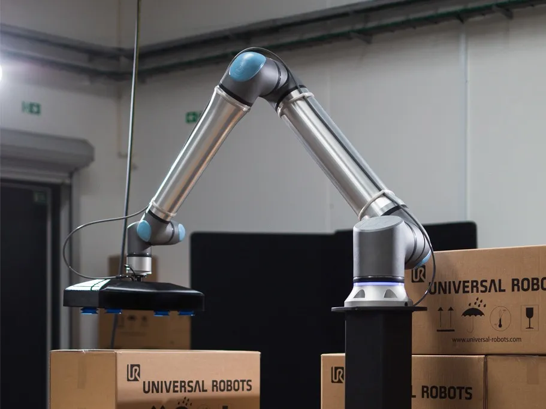
\includegraphics[width=0.60\textwidth]{images/UR20}
    \caption{UR20 Palletizing concept image}
\end{figure}
\newpage
\section{Product Description}
This section provides the reader with an overview of UR20. The primary operational aspects of the product, from the perspective of end users, maintainers and administrators, are defined here. The key features and functions found in the product, as well as critical user interactions and user interfaces are described in detail.

\subsection{Features \& Functions}
The UR20 will perform a palletizing application using an added vacuum gripper to the end of the arm as well as a QR code reader that will store the package information, such as where it needs to be placed. Once the data is processed, the arm will place the box according to its size. As seen in the system, the griper will be made up of 20 bellow cup suction gripers  attached to an air compressor

\subsection{External Inputs \& Outputs}
The UR20 will perform a palletizing application with an added vacuum gripper at the end of the arm. The data needed to process this palletizing application will be the QR code that will communicate via serial communication to the robot arm. This information will be processed by the robot arm's code, which will contain information such as the size and position of the box needed to be placed in the pallet. The vacuum gripper will be used to pick up the box. The UR20 will be used to move the object to the apparatus location. This QR code reader will store the package information, such as where to place it. Once the data is processed, the arm will place the box accordingly. 

\subsection{Product Interfaces}
The end user will have access to a Teach Pendant which is a tablet-like screen that can be used to do maintenance on the UR20. From this tablet, one can program the robot, run a program, or configure robot installation. This allows for easy adjustments to the UR20's behavior.
\newpage
\section{Customer Requirements}
This section outlines the customer requirements for the UR20 robotic arm to palletize uniform sized boxes, each marked with a QR code containing box dimensions. The porject also includes the design and implementation of a custom robotic gripper that incorporates bellow suction cups to handle the boxes effectivelty. The robot arm will maintain full functionality in scanning the QR code and locating the box, picking it up and placing on a pallet. 
\subsection{Box Palletizing by UR20 Robot}
\subsubsection{Description}
The UR20 will be used to palletize boxes based on model 1 QR codes, process data, and stack boxes in an effective manner. The system will handle boxes of the same size, ensuring precise and efficient stacking.
\subsubsection{Source}
 CSE Senior Design project specifications
\subsubsection{Constraints}
Environment is suitable for operation of collaborative robot in a safe manner. QR codes are readable with minimal stains, spots, or missing data.
\subsubsection{Standards}
ISO 10218-1 Robots and robotic devices — Safety requirements for industrial robots ensuring protective measures.
ISO 10218-2, Robots for industrial environments – Safety requirements to minimize hazards associated with robots and end effectors.
\subsubsection{Priority}
Critical
The priority of this requirement relative to other specified requirements. Use the following priorities:

\subsection{Custom Gripper with Vacuum and Bellow Cups}
\subsubsection{Description}
The gripper design will feature bellow cups and a vacuum to securely handle and move the boxes during the palletizing process. It will be designed to fit the size of the boxes and ensure firm grasping tro prevent slippage during handling.
\subsubsection{Source}
CSE Senior Design Project specifications
\subsubsection{Constraints}
The strength and durability of the bellow cups support the box weight, selection of materials for sustainability.
\subsubsection{Standards}
ISO/TR 20218-1:2018 Robotics — Safety design for industrial robot systems, ensuring safety measures for design and integration of end-effectors.
ISO 10218-2, Robots for industrial environments – Safety requirements to minimize hazards associated with robots and end effectors.
\subsubsection{Priority}
High
\newpage
\section{Packaging Requirements}
The packaging requirements for the UR20 robot and custom-designed gripper will include pre-installed control software. Additionally, the custom gripper will be fully assembled and contained in a single package. The requirements focus on making the product easily deployable and ready for use in palletizing operations.
\subsection{Pre-Installed Software}
\subsubsection{Description}
The control software for operating the UR20 robot will be pre-installed on the the system before delivery to the customer. The robot can immmediately perform palletizing application upon arrival without complex installation procedures. 
\subsubsection{Source}
CSE Senior Design Project Specifications
\subsubsection{Constraints}
The software must be compatible with the UR20 system and ensure reliable functionality. Limited modifications will be needed by customer post-installation.
\subsubsection{Standards}
ISO/IEC/IEEE 12207:2017 Systems and software engineering — Software life cycle processes - proper installation and support for future updates
\subsubsection{Priority}
High
\subsection{Gripper Assembly and Packaging}
\subsubsection{Description}
The gripper mechanism, including vacuum suction cups, will be delivered pre-assembled and tested for immediate use with the UR20 robot. All components will be securely packaged to avoid damage during transportation. 
\subsubsection{Source}
CSE Senior Design Project Specifications
\subsubsection{Constraints}
The packaging must ensure the safe transport of the assembled gripper, sourcing of packaging material will be the responsibility of the engineering team.
\subsubsection{Standards}
ISO 3676:2012 Packaging — Complete, filled transport packages and unit loads — Unit load dimensions ensuring products arrive safely from their origin to their destination.
\subsubsection{Priority}
High
\newpage
\section{Performance Requirements}
This section defines the preformance requirements that the UR20 will need to meet. 

\subsection{palletizing speed}
\subsubsection{Description}
The UR20 will be able to place boxes in a timely manner while being fed boxes through a conveyor belt 
\subsubsection{Source}
LJCJ Team Decision
\subsubsection{Constraints}
Pallet size restriction of 40''X48''
\subsubsection{Standards}
GMA pallet standards
\subsubsection{Priority}
High

\subsection{Box Size}
\subsubsection{Description}
The UR20 will be able to pick up boxes of size 12''X20'' 
\subsubsection{Source}
LJCJ Team Decision
\subsubsection{Constraints}
Maximum payload of 20kg 
\subsubsection{Standards}
NO standard applicable
\subsubsection{Priority}
Moderate

\subsection{QR Box Reading}
\subsubsection{Description}
The UR20 will be able to read the next box QR code prior to picking up the box 
\subsubsection{Source}
LJCJ Team Decision
\subsubsection{Constraints}
Box mut be in a proper orientation for the QR to be visible
\subsubsection{Standards}
NO standard applicable
\subsubsection{Priority}
Moderate

\subsection{Sucessful box placement rate}
\subsubsection{Description}
 Less than 10\% of baxes must be droped or missplaced
\subsubsection{Source}
LJCJ Team Decision
\subsubsection{Constraints}
Gripper must have proper allignment and force to carry and place Box
\subsubsection{Standards}
NO standard applicable
\subsubsection{Priority}
High

\newpage
\section{Safety Requirements}
This section defines the safety standards that will taken when the UR20 is operating. The UR20 is a collaborative robot, commonly known as a Cobot, meaning that human collaboration with the Cobot is possible when safety guidelines are followed. Although this robot is deemed 'collaborative', it is not entirely safe for humans. Injuries from electrical shock, impact, or compression can still occur if proper safety measures are not taken. In this use case, the UR20 will be transporting cardboard boxes of a consistent weight between a pallet and a conveyor belt, which could impact or crush the human user not taking proper precautions.

\subsection{Laboratory equipment lockout/tagout (LOTO) procedures}
\subsubsection{Description}
Any fabrication equipment provided used in the development of the project shall be used in accordance with OSHA standard LOTO procedures. Locks and tags are installed on all equipment items that present use hazards, and ONLY the course instructor or designated teaching assistants may remove a lock. All locks will be immediately replaced once the equipment is no longer in use.
\subsubsection{Source}
CSE Senior Design laboratory policy
\subsubsection{Constraints}
Equipment usage, due to lock removal policies, will be limited to availability of the course instructor and designed teaching assistants.
\subsubsection{Standards}
Occupational Safety and Health Standards 1910.147 - The control of hazardous energy (lockout/tagout).
\subsubsection{Priority}
Critical

\subsection{National Electric Code (NEC) wiring compliance}
\subsubsection{Description}
Any electrical wiring must be completed in compliance with all requirements specified in the National Electric Code. This includes wire runs, insulation, grounding, enclosures, over-current protection, and all other specifications.
\subsubsection{Source}
CSE Senior Design laboratory policy
\subsubsection{Constraints}
High voltage power sources, as defined in NFPA 70, will be avoided as much as possible in order to minimize potential hazards.
\subsubsection{Standards}
NFPA 70
\subsubsection{Priority}
Critical

\subsection{RIA robotic manipulator safety standards}
\subsubsection{Description}
Robotic manipulators, if used, will either housed in a compliant lockout cell with all required safety interlocks, or certified as a "collaborative" unit from the manufacturer.
\subsubsection{Source}
CSE Senior Design laboratory policy
\subsubsection{Constraints}
Collaborative robotic manipulators will be preferred over non-collaborative units in order to minimize potential hazards. Sourcing and use of any required safety interlock mechanisms will be the responsibility of the engineering team.
\subsubsection{Standards}
ANSI/RIA R15.06-2012 American National Standard for Industrial Robots and Robot Systems, RIA TR15.606-2016 Collaborative Robots
\subsubsection{Priority}
Critical

\subsection{Collaborate robot industrial safety requirements}
\subsubsection{Description}
Collaborative robots remain dangerous, and collaborators entering the work area of a Co-bot shall adhere to specific safety requirements in order to prevent bodily harm. 
\begin{enumerate}
  \item The movement path of the collaborator(s) must be kept free of tripping or other movement hazards while the Cobot is powered on.
  \item A collaborator shall not enter the workspace with dangling jewelry, loose clothing, or long loose hair.
  \item Collaborator(s) must not enter the marked Cobot operating space while the Cobot is active.
\end{enumerate}
\subsubsection{Source}
International Organization for Standardization
\subsubsection{Constraints}
    Those not adhering to the safety requirements listed in ISO/TS 15066 shall be prohibited from collaboration with the Cobot until adherence to the requirements resumes.
\subsubsection{Standards}
ISO/TS 15066:2016
\subsubsection{Priority}
High

\subsection{Collaborate robot workspace clearance requirements}
\subsubsection{Description}
The collaborative robot workspace should be clear of hazards that could impede the movement of the collaborator(s) or the Cobot itself.  
\begin{enumerate}
  \item The collaborative space of the Cobot, where humans are safe to interact, must be visibly delineated from the operating space of the Cobot.
  \item The Cobot shall function with reduced force when a human is present. In calculating these reduced forces, the weight of the payload must be considered.
  \item The workspace of the Cobot must be kept free of blockages or other movement hazards while the Cobot is powered on.
  \item Possible locations of quasi-static contact (where a human may be clamped between any part of the Cobot and the working environment, including another part of the Cobot) must be identified and removed where possible.
  \item Possible locations of transient contact (where the Cobot or the environment may collide with a human) must be identified and removed where possible. The force of contact should also be considered.
\end{enumerate}
\subsubsection{Source}
International Organization for Standardization
\subsubsection{Constraints}
    Not all possible locations of contact will be removeable. To account for this, dangerous areas must be delineated as part of the Cobot operating space. Risk of injury at these locations shall be minimized by calculating the reduced force used by the Cobot according to ISO 10218-1:2011.
\subsubsection{Standards}
ISO/TS 15066:2016 and ISO 10218-1:2011
\subsubsection{Priority}
High


\subsection{Force adjustment according to dynamic item weight}
\subsubsection{Description}
The collaborative robot will adjust the force it uses dynamically according to the weight of the item, as opposed to assuming a uniform weight for all items.
\subsubsection{Source}
International Organization for Standardization
\subsubsection{Constraints}
Judging the weight of the item would be difficult, and somewhat out of scope for this project. A weighing system would have to be implemented, either negatively accounting for weight leaving the conveyor belt or implemented directly in the robot arm itself.
\subsubsection{Standards}
ISO/TS 15066:2016 and ISO 10218-1:2011
\subsubsection{Priority}
Future

\newpage
\section{Security Requirements}
This section defines the security standards that will be taken to avoid malicious tampering involving the hardware or software of the Cobot. In the event that the Cobot's security is confirmed to be compromised, continued use will be halted until approval is given by the course instructor.

\subsection{Physical Security}
\subsubsection{Description}
The Cobot, including the programming tools and control systems, shall be located in an area that only approved persons may access. In the event that an unapproved person gains access to the Cobot, the possibility of tampering should be ruled out for both the hardware and software of the Cobot.
\subsubsection{Source}
LJCJ Team Decision
\subsubsection{Constraints}
The Senior Design lab is frequently used by a large number of students. As it would be impossible work in the case that all of those students were considered a safety concern, these studenst shall be considered approved persons.
\subsubsection{Standards}
N/A
\subsubsection{Priority}
High

\subsection{Cyber Security}
\subsubsection{Description}
In the event that network access is necessary, the Cobot should not be connected to insecure or unknown networks. When connection is no longer needed, the Cobot should be disconnected from the network.

Similarly, the Cobot should not be connected to insecure or unknown devices.

Removeable media shall only be used when its contents are completely known and approved of by at least one member of the team. Do not insert removeable media of dubious origin into the Cobot. 
\subsubsection{Source}
LJCJ Team Decision
\subsubsection{Constraints}
The Cobot may need to be connected to UTA Wi-Fi and our team's computers, which are not very secure. However, it is unlikely that the course instructor will fund alternatives, so these must be used regardless. 
\subsubsection{Standards}
N/A
\subsubsection{Priority}
High
\newpage
\section{Maintenance \& Support Requirements}
Maintenance and support requirements define the necessary measures to ensure that the UR20 robotic palletizing system remains fully functional after deployment. Effective support includes troubleshooting guides and accessible source code for any required modifications. Additionally, maintenance teams must be equipped with appropriate tools to service the robot system.

\subsection{Maintenance Procedures for UR20 and Conveyor System}
\subsubsection{Description}
Routine maintenance must be performed on the UR20 robot and the conveyor system to ensure proper functionality. This included for wear and tear on the bellow cups, the end effector itself, the robot arm, and conveyor belt mechanism.
\subsubsection{Source}
LJCJ Team
\subsubsection{Constraints}
Constraints include the availability of spare parts and in case of gripper needing full repair the design schematics will be provided. 
\subsubsection{Standards}
ISO 9283:1998 Manipulating industrial robots — Performance criteria and related test methods for industrial robots
ISO 10218-1:2011 Robots and robotic devices — Safety requirements for industrial robots 
\subsubsection{Priority}
High

\subsection{Support Documentation and Troubleshooting Guides}
\subsubsection{Description}
Detailed troubleshooting manuals and user guides will be provided based on the team's experience when working with the UR20. This will include known issues that may arise and step-by-step instructions on how to resolve them. Digital access to the resources will be available.
\subsubsection{Source}
LJCJ Team
\subsubsection{Constraints}
Documentation must be kept up to date with any changes to the system. such as software updates or any change in hardware. 
\subsubsection{Standards}
IEEE 1063-2001 IEEE Standard for Software User Documentation - content on the software will be provided to the user and meets proper documentation practices
\subsubsection{Priority}
High

\subsection{Source Code availability }
\subsubsection{Description}
The source code for the UR20 control system will be available to maintainers for debugging and future updates. A version control system will be utilized to track changes in the software and maintain organization. 
\subsubsection{Source}
LJCJ Team
\subsubsection{Constraints}
Constraints include ensuring the version control system is maintained properly, only allowing authorized users to modify code.
\subsubsection{Standards}
ISO/IEC/IEEE International Standard - Software engineering - Software life cycle processes - Maintenance (maintain software)
\subsubsection{Priority}
High


\newpage
\section{Other Requirements}
The UR20 in a palletizing application will require a conveyor belt, vacuum gripper attachment, and E-stop button. These components must be configured to work with the UR20 and each other for each new environment and job (with the exception of the E-stop button, which will always perform the same task in every situation).

\subsection{E-stop button}
\subsubsection{Description}
The E-Stop will completely halt all operations of the UR20, conveyor belt, and vacuum generator. 
\subsubsection{Source}
LJCJ Team Decision
\subsubsection{Constraints}
Some components may not take kindly to having the power cut unexpectedly. This should be considered before testing of the E-stop button begins.
\subsubsection{Standards}
N/A
\subsubsection{Priority}
Critical

\subsection{Vacuum Gripper Attachment}
\subsubsection{Description}
A vacuum gripper must be constructed in order for the UR20 to fulfill its basic purpose. Once built, it shall provide appropriate suction power in order to securely transport a box, and a release of that suction in order to deposit the box.
\subsubsection{Source}
LJCJ Team Decision
\subsubsection{Constraints}
The vacuum gripper's completion date is dependent on shipping times and the success of prototypes.
\subsubsection{Standards}
N/A
\subsubsection{Priority}
Critical

\subsection{Conveyor Belt}
\subsubsection{Description}
The conveyor belt must be configured to operate at a suitable speed, one that can keep up with the UR20's max speed while not spilling over when the UR20 slows down to accommodate a human presence. It must be placed in a location that is marked, as if its position significantly changes the UR20 may have difficulty recognizing the boxes.
\subsubsection{Source}
LJCJ Team Decision
\subsubsection{Constraints}
This is dependent on the conveyor belt's adjustability. In the case that a variable speed cannot be achieved, the UR20 may be forced to operate at a low speed at all times.
\subsubsection{Standards}
N/A
\subsubsection{Priority}
Moderate
\newpage
\section{Future Items}
\subsection{Force adjustment according to dynamic item weight}
\subsubsection{Description}
The collaborative robot will adjust the force it uses dynamically according to the weight of the item, as opposed to assuming a uniform weight for all items.
\subsubsection{Source}
International Organization for Standardization
\subsubsection{Constraints}
Judging the weight of the item would be difficult, and somewhat out of scope for this project. A weighing system would have to be implemented, either negatively accounting for weight leaving the conveyor belt or implemented directly in the robot arm itself.
\subsubsection{Standards}
ISO/TS 15066:2016 and ISO 10218-1:2011
\subsubsection{Priority}
Future

\subsection{Depallatizing aplication of the UR20}
\subsubsection{Description}
The collaborative robot will implement a Depalletizing application with the same hardware. The addition would be using computer vision to detect the boxes and the approach to deputizing.
\subsubsection{Source}
Source
\subsubsection{Constraints}
Computer vision and the ability to decide the order in which boxes were placed prior will be difficult to implement, given the time Constraints.
\subsubsection{Standards}
CoaXPress – Hosted by JIIA; release date 2010; current version 2.1
Camera Link HS – Hosted by A3; release date 2012; current version 1.2
IIDC2 – Hosted by JIIA; release date 2012; current version 1.1.0
USB3 Vision – Hosted by A3; release date 2013; current version 1.2
\subsubsection{Priority}
Future

\subsection{palletizing without using QR codes}
\subsubsection{Description}
The collaborative robot will have implement computer vision to determine box placement
\subsubsection{Source}
LJCJ Team Desicion
\subsubsection{Constraints}
Insufficent time to implement a computer vision aglgorithm for paletizing
\subsubsection{Standards}
no applicable standards
\subsubsection{Priority}
Future

\subsection{palletizing boxes of difrent size}
\subsubsection{Description}
The collaborative robot will implement a visions algorithm to place diffrent items onto a pallet
\subsubsection{Source}
LJCJ Team Desicion
\subsubsection{Constraints}
Insufficent time to implement a computer vision aglgorithm for paletizing
\subsubsection{Standards}
no applicable standards
\subsubsection{Priority}
Future
\newpage

%%% References
\bibliographystyle{plain}
\bibliographystyle{reference/IEEEtran_custom}
\bibliography{reference/refs}{}

\end{document}